\documentclass[12pt,oneside,a4paper,english]{article}
\usepackage[T1]{fontenc}
\usepackage[utf8]{inputenc}
\usepackage[margin=2.25cm,headheight=26pt,includeheadfoot]{geometry}
\usepackage[english]{babel}
\usepackage{listings}
\usepackage{color}
\usepackage{titlesec}
\usepackage{titling}
\usepackage[framed, numbered]{matlab-prettifier}
\usepackage{changepage}
\usepackage{amsmath}
\usepackage{amssymb}
\usepackage{hyperref}
\usepackage{enumitem}
\usepackage{graphicx}
\usepackage{fancyhdr}
\usepackage{lastpage}
\usepackage{caption}
\usepackage{tocloft}
\usepackage{setspace}
\usepackage{multirow}
\usepackage{titling}
\usepackage{float}
\usepackage{comment}
\usepackage{booktabs}
\usepackage{indentfirst}
\usepackage{lscape}
\usepackage{booktabs,caption}
\usepackage[flushleft]{threeparttable}
\usepackage[english]{nomencl}
\usepackage{xcolor}
\usepackage{lipsum}
\usepackage{tikz}
\usepackage[final]{pdfpages}
\usepackage{graphicx}
\usepackage{resizegather}
\usepackage{tabularx}
\usepackage[numbers]{natbib}
\usepackage{verbatim}

\usepackage{xcolor}
\usepackage{listings}

% Define Cucumber language settings
\lstdefinelanguage{cucumber}{
  morekeywords={Feature, Scenario, Given, When, Then, And},
  keywordstyle=\color{blue},
  sensitive=false,
  morecomment=[l]{\#},
  morestring=[b]',
  morestring=[b]",
}

% Define a custom style for Cucumber code
\lstdefinestyle{cucumberstyle}{
  basicstyle=\ttfamily\small,
  breaklines=true,
  frame=single,
  numbers=left,
  numberstyle=\tiny\color{gray},
  stepnumber=1,
}




% --- set footer and header ---
\pagestyle{fancy}
\fancyhf{}

\setlength{\parindent}{2em}
\title{Report 1 - Group 9} % to reference as \title, dont use \maketitle
\makeatletter\let\Title\@title\makeatother



\lstset{language=Matlab,
style=Matlab-editor,
basicstyle=\normalsize\mlttfamily,
numbers=left,
numberstyle={\scriptsize\color{black}},			% size of the numbers
numbersep=0.5cm											
}
\lstset{language=cucumber, style=cucumberstyle}


\newlist{steps}{enumerate}{1}
\setlist[steps, 1]{leftmargin=1.5cm,label = Step \arabic*:}
\renewcommand{\headrulewidth}{1pt}
\renewcommand{\footrulewidth}{1pt}

%\lhead{\Title}
\rhead{\nouppercase{\rightmark}}
\lhead{\Title}
\rfoot{
\includegraphics[height=1.25cm]{root/logo.pdf}} % right header logo
\setlength\headheight{16pt}
\setlength{\footskip}{50pt}
\lhead{\Title} %rightH title
\cfoot{\thepage}

\setcounter{tocdepth}{4}
\setcounter{secnumdepth}{3}


% --- End of page settings ---



\begin{document}
\pagenumbering{roman} 

\begin{titlepage}
\begin{center}
\vspace{2cm}
%\textsc{ Danmarks Tekniske Universitet}\\[1.5cm]

\includegraphics[width=0.4\textwidth]{root/dtu.png}~\\[1cm]

% Title
\hrule
\vspace{.5cm}
{ \huge \bfseries Requirements Specification and Program Design\\} % title of the report
\vspace{.5cm}
{ \bfseries Software Engineering 1 | 02161\\}
{ \bfseries Exam Project Report: Part 1 | Group 9}
\vspace{.5cm}

\hrule
\vspace{.5cm}

\includegraphics[width=0.5\textwidth]{figures/indsæt_billede.jpeg}

\vspace{0.5cm}

\textsc{\textbf{Authors}}\\
\vspace{.5cm}
\centering

% add your name here
Charlotte Ena Manikutdlak Grimstrup - s204382\\
Emil - s194501\\
Max-Peter Schrøder - s214238\\
Sebastian Alberg Ladegaard - s215530\\
Simon - s214751

\vspace{0.5cm}

\centering \today % Dags dato
\end{center}
\end{titlepage}

\newpage
\doublespacing
%\addcontentsline{toc}{section}{Table of Contents}
\renewcommand{\baselinestretch}{1}\normalsize
\tableofcontents
\renewcommand{\baselinestretch}{1}\normalsize
%\singlespacing
\thispagestyle{fancy} % force page style

\newpage
\pagenumbering{arabic} 
\fancyfoot[C]{Page \thepage\ of \pageref{EndOfText}}

\section{Requirements specification} \label{ch1}
% Indledning: Dette afsnit skal indeholde en kort indledning og opsummering afbesvarelsen.
\subsection{Introduction}



%Væsentlige begreber (ordliste, glossar): Dette afsnit skal indeholde en opremsning af de væsentlige begreber fra problem domænet. Hvert begreb gives en kort definition på nogle få liner. OBS: der kræves ingen domæneklassediagram. Dvs. klassediagram som viser problem domain
\subsection{Essential Concepts}
This section showcases the essential concepts of the project domain in a glossary.

\subsubsection{Glossary}  % jeg lavede et overflødigt subsubsection fordi jeg gerne vil ehave paragraphs i table of content i pdf filen, og pdffiler kan ikke håndtere at springet fra subsection til paragraph... Det lidt grimt... men jeg vil gerne have muligheden for at navigere til specifikke elementer i table of content i pdf-filen.
\paragraph*{Softwarehuset A/S:} A company which consists of around 50 employees and has 30 ongoing projects, which is in need of a new project management system.
\paragraph*{Project management system:} A system to manage projects and time registration for Softwarehuset A/S. The system is internal, so no password control is needed for access, only employee initials.
\paragraph*{Project:} A project contains selection of activities. A project is created when a major task needs to be done. A project needs a name, and an ID defined by the system, in the form year and number, for example 22001 , 22002, etc. Each project can have an assigned project manager with special privileges. A project can be ordered by a costumer, or be an internal project made for Softwarehuset A/S. A project typically has 30 activities, but some have upwards of 100.
\paragraph*{Project activity:} A project activity is a task assigned to a project. For each activity, the project manager can define the expected working hours for completion, as well as set a starting date and a project duration (in weeks) The duration of an activity is typically 2-3 weeks.
\paragraph*{Non-project activity:} An activity not related to a project, such as sick days, holidays, courses and more. These are created by employees themselves, and set with a name which combines their employee ID, as well as a date and duration (in days).
\paragraph*{Employee:} Development staff member at Softwarehuset A/S, designated in the system with their initials (up to 4 characters), for example huba, ahad, ekki, etc. An employee can be assigned an activity by a project manager, and has to self-register the amount of time used on all active activities on a daily basis. An employee typically works on less than 10 activites during a week, but some employees are allowed to work on up to 20 activities during a week. At the end of the day, an employee has to register the amount of time worked on a specific activity via a time registration ticket. An employee can only work up to 8 hours on a working day.
\paragraph*{Project manager:} An employee can assign themselves as manager of a specific project. Project managers have exclusive rights to create, edit and remove activities from their projects, and can assign employees to activities, where they can see all available employees to assign. They can also set a starting-week, activity duration (in weeks) and expected workload, to determine the ending-week and weekly workload needed. They can further see how the time spent on activities and the project are proceeding, as well as how much work is still needed, and generate project reports for meetings.
\paragraph*{Project registration:} Interaction with system to register projects. Projects can be registered by an employee, who must define a name and an ID. No project manager, starting week, duration or expected workload are assigned to the project when it is created.
\paragraph*{Activity registration:} Interaction with system to register activities. Activities for a project can be created by the assigned project manager. If no project manager is assigned to a project, an employee may create project activities, but cannot set the expected workload, starting week and duration, that is beholden to the project manager. Employees can always create non-project activities, and set their starting day, week and year, and duration.
\paragraph*{Time registration ticket:}  A note containing amount of time used on a particularly activity on a particular day in 1/2 hour precision. An employee has to create these tickets at the end of the day. Employees can edit their registrations.
\paragraph*{Employee activity assignment:} Project leaders can assign one or multiple employees to an activity. When that happens, the expected workload is divided by the activity duration (in weeks) to produce an expected weekly workload for the employee(s).
\paragraph*{Expected workload:} Expected hours to complete a project or an activity, set by the project manager.
\paragraph*{Starting date:} A date indicating the starting time for a project or activity. For projects and project activities, the starting date is always the first day of a week. For non-project activities, the starting date can be any workday of a week.
\paragraph*{Duration:} Indicates the duration of a project or an activity. For projects and project activities, the duration is always in working weeks. For non-project activities, the duration is always in working days.
\paragraph*{Project reports:} A report generated by the project manager. The project manager can choose to generate a report for a given activity (using the name and furthermore the ID for disambiguation if needed), which contains the amount of time worked on that activity and also which employees spend that time, optionally he can create a day by day overview of the time spend on that activity. The project manager can also generate a report for a project, which contains the total amount of time spent on that project and which employees spend that time, optionally he can create a week by week overview of the time spend on that activity.


%Dag i uge, uge og år
%Project: første dag i ugen, uge, år og duration (uger)
%Project activity: første dag i ugen, uge, år og duration (uger)
%Non-project activity: bestemt dag i uge, uge, år og duration (dag)


% Medarbejder:
% - skal (hvis der ikke er projektleder på) gradvis opdele projektet i aktiviteter
% - 

% Projektlederen: (Kan alt hvad medarbejderen kan)
% - skal gradvist opdele projektet i aktiviteter
% - For hver aktivitet skal projektlederen kunne anføre forventet antal arbejdstimer til løsning af opgaven (budgetteret tid)
% - Endvidere skal der kunne anføres start- og sluttid på aktiviteten

% Aktivitet: 
% - Budget ( i timer )
% - starttid/sluttid (ugenummer)




%Use case diagram: Dette afsnit skal give en beskrivelse af de væsentlige operationeri form af et use case diagram. Hvis et use case diagram bliver uoverskueligt, kan derogs˚a bruges flere use case diagrammer. Husk et form˚alet af use case diagrammerer et skabe en oversigt over programmernes funktionalitet.
\subsection{Use Case Diagram}
The below use case diagram showcases all general user interactions with the 

A project manager is an extension of an employee, so all employee use cases also apply to project managers, but not the other way around.



%Detaljeret use cases Der skal ogs˚a være detaljeret use cases med hoved– og al-ternative/fejl scenarier som Cucumber features. Der skal være 2 detaljeret usecases/Cucumber features til hver medlem i gruppen (dvs. 8 for firmandsgrupperog 10 for femmandsgrupper).
\subsection{Detailed Use Cases}

\begin{itemize}
    \item As an employee:
    \begin{itemize}
        \item I want to be able to register time spent working on an activity on a given day.
        \item I want to be able to create a project with a name and an ID.%Max 1
        \item I want to be able to create a non-project activity and give it a starting date and expected duration. %Sebastian #2
        \item I want to be able to set myself as project manager - for a project that doesn't have a manager - and set starting week, duration and expected workload %Max 2
    \end{itemize}
    
    \item As an employee, given that there is no project manager on a project, I want to be able to register an activity on said project ( But not be able to set expected workload, starting week and duration) 


    \item As a project manager for a given project, I want to be able to:
    \begin{itemize}
        \item create an activity in said project with expected workload as well as a starting date and a project duration. %Sebastian #1
        \item edit an activity in said project.
        \item remove an activity in said project. %Emil #1
        \item assign an employee to an activity in said project (given that the employee is assigned to less than 20 activities for the given weeks). %Emil %2
    \end{itemize}

    
    \item As a project manager, I want to be able to view the employees who are available during the time designated for an activity.

    \item as a project manager, I want the system to create a detailed report of my project, which will easy my workload %Sebastian #3


    
\end{itemize}



% 
%All 10 features we chose:
%1. Login to the system.
%2. Create a new project with a name and an ID. 
%3. Create a non-project activity and give it a starting date and expected duration.
%4. Register time spent working on an activity on a given day, even if I haven't been specifically assigned to that activity.
%5. Set myself as project manager - for a project that doesn't have a manager - and set starting week, duration and expected workload.
%6. Edit the project.
%7. Create an activity in said project with starting date, duration and expected workload.
%8. Assign an employee to an activity in said project.
%9. View the employees who are available to be assigned during the time designated for an activity.
%10. Create a detailed report of my project, which showcases relevant metrics for evaluation.


\subsubsection{Feature 1: Login to the system} %Emil 1
%1. Login to the system. DONE
\begin{lstlisting} 
Feature: Login to the system #Emil 1
    Description: Login into the system
    Actor: Employee

Scenario: Employee logs in
    Given that no-one is logged in
    And an employee with an ID exists
    When an employee logs in with their ID
    Then the employee is logged into the system

Scenario: Employee does not exists
    Given that no-one is logged in
    And an employee has an ID that is not registered in the system
    When an employee logs in with the ID
    Then the employee is not logged into the system, and an error message "Employee ID does not exist" appears
\end{lstlisting}

\subsubsection{Feature 2: Create a new project}%Max 1
%2. Create a new project with a name and an ID. DONE
\begin{lstlisting}
Feature: Create a new project # Max 1
    Description: Create a new project with a name and generated ID
    Actor: Employee

Scenario: New project is created
    Given an employee is logged in
    And the current date is in the year 2024
    When the employee creates a new project with the name "TestProject"
    Then a project with the name "TestProject" and ID "24XYZ" is created, where XYZ is the number of the project

Scenario: Project name already exists
    Given an employee is logged in
    And the current date is in the year 2024
    And a project with the name "TestProject" exists
    When the employee creates a new project with the name "TestProject"
    Then the project is not created, and an error message "Project already exists" appears
\end{lstlisting}

\subsubsection{Feature 3: Create non-project activity} %Charlotte 1
%3. Create a non-project activity and give it a starting date and expected duration. DONE
\begin{lstlisting}
Feature: Create non-project activity # Seb 2
    Description: Creating a non-project activity
    Actor: Employee

Scenario: Create a non-project activity
    Given an employee is logged in
    And there is an activity with the name "Vacation" 
    And the activity starts on a given day with a duration of "14" days
    When the employee creates the non-project activity
    Then the non-project activity is created

Scenario: Create a non-project activity that already exists
    Given an employee is logged in
    And there is an activity with the name "Vacation"
    When the employee creates a non-project activity with the name "Vacation"
    Then the error message "Non-project activity already exists" appears
\end{lstlisting}

\subsubsection{Feature 4: Register time spent on activity} 
%4. Register time spent working on an activity on a given day, even if I havent been specifically assigned to that activity. DONE
\begin{lstlisting}
Feature: Register time spent on activity  # Simon 1
    Description: Register the time spent on an activity on the given day
    Actor: Employee

Scenario: Register time for a project activity
    Given the employee is logged in
    And it is the current date
    And an activity with the name "TestActivity" exists in project "TestProject"
    When the employee registers "9" half-hours spent on the activity
    Then the time spent by the employee is registered to the activity and the employee

Scenario: Register time for non-project activity
    Given the employee is logged in
    And there is an activity with the name "Vacation" 
    When the employee employee registers "5" days spent on the non-project activity
    Then the time spent by the employee is registered to the non-project activity and the employee

Scenario: Edit project activity time registration
    Given the employee is logged in
    And an activity with the name "TestActivity" exists in project "TestProject"
    And the employee has previously registered time on this activity
    When the employee edits the time spent on the activity for this registration
    Then the time registration ticket is updated for the employee and the activity

Scenario: Edit time for non-project activity
    Given the employee is logged in
    And there is an activity with the name "Vacation"
    When the employee edits the duration in days spent on the non-project activity
    Then the time spent by the employee is registered to the non-project activity and the employee
\end{lstlisting}


\subsubsection{Feature 5: Set project manager for a project}%Max 2
%5. Set myself as project manager - for a project that doesn't have a manager DONE
\begin{lstlisting}
Feature: Set project manager for a project # Max 2
    Description: An employee assigns themselves as project manager for an unassigned project
    Actor: Employee / Project manager

Scenario: Self-assign as project manager
    Given an employee is logged in
    And a project with the name "TestProject" exists
    When the employee self-assigns themselves as project manager of the project
    Then they become the project manager of the project
    
Scenario: Project manager is already assigned
    Given an employee is logged in
    And a project with the name "TestProject" exists
    And the project has an existing project manager
    When the employee self-assigns themselves as project manager of the project
    Then they do not become the project manager, and an error message "Project already has an assigned project manager" appears
\end{lstlisting}

\subsubsection{Feature 6: Edit project}
%6. Edit the project DONE
\begin{lstlisting}
Feature: Edit project # Simon 2
    Description: Set and edit the parameters of a project
    Actor: Project manager

Scenario: Set project parameters
    Given an employee is logged in
    And he is the project manager of a project "TestProject"
    When the project manager sets the starting week as "5", the duration as "3" weeks, the year as "2024", and expected workload as "200" hours
    Then the project has these parameters set

Scenario: Change project parameters
    Given an employee is logged in
    And he is the project manager of a project "TestProject"
    And the project has a set starting week, duration and expected workload
    When the project manager updates the parameters
    Then the project parameters are changed

Scenario: Change name of project
    Given an employee is logged in
    And he is the project manager of a project "TestProject"
    When he changes the name of the project to "TestProject2"
    Then the name of the project is changed to "TestProject2"

Scenario: Change project name but already exists
    Given an employee is logged in
    And he is the project manager of a project "TestProject"
    And another project exists with the name "TestProject2"
    When the project manager changes the name to "TestProject2"
    Then the project name is not changed and an error message "This project name already exists as a separate project" appears
\end{lstlisting}

\subsubsection{Feature 7: Create project activity} %Charlotte 2
%7. Create an activity in said project with starting date, duration and expected workload DONE
\begin{lstlisting}
Feature: Create project activity # Seb 1
    Description: Creating an activty and setting the parameters
    Actor: Project manager

Scenario: Create a project activity
    Given the employee is logged in
    And he is the project manager of a project "TestProject"
    When he creates a project activity "TestActivity" in the project
    Then the project activity is created

Scenario: Change project activity name but already exists
    Given an employee is logged in
    And the employee is the project manager of a project "TestProject"
    And an activity with the name "TestActivity" exists in the project
    When the employee creates an activity in the project with the name "TestActivity"
    Then the project activity is not created, and an error message "This project activity name already exists as a activity" appears
 \end{lstlisting}   

\subsubsection{Feature 8: Assign an employee to a project activity}
%8. Assign an employee to an activity in said project. DONE
\begin{lstlisting}
Feature: Assign an employee to a project activity # Emil 2
    Description: The act of assigning an employee to a project activity
    Actor: project manager

Scenario: Assign employee to project activity
    Given an employee is logged in
    And the employee is the project manager of a project "TestProject"
    And an activity with the name "TestActivity" exists in the project
    When the project manager assigns an employee to the project activity
    The employee is assigned to the project activity

Scenario: Employee is unavailable for activity
    Given an employee is logged in
    And the employee is the project manager of a project "TestProject"
    And an activity with the name "TestActivity" exists in the project
    And another employee exists, who cannot take on more activities currently
    When the project manager assigns an employee to the project activity
    Then the employee is not assigned to the project activity
    And an error message "Employee cannot currently take on more activities" appears

Scenario: project does not exist

Scenario: Activity does not exist
    Given an employee is logged in
    And the employee is the project manager of a project "TestProject"
    And no activity with the name "TestActivity" exists in the project
    When the project manager tries to assign an employee to the activity
    Then an error message "Activity does not exist in the given project"

Scenario: Employee is already assigned to the activity
    Given an employee is logged in
    And the employee is the project manager of a project "TestProject" 
    And an activity with the name "TestActivity" exists in the project
    And another employee is already assigned to the activity
    When the project manager assigns the other employee to "TestActivity"
    Then the other employee is still assigned to "TestActivity" and an error message "This employee is already assigned to this activity" appears

Scenario: Not project manager for given project
    Given an employee is logged in
    And the employee is not the project manager of a project "TestProject" 
    And an activity with the name "TestActivity" exists in the project
    When the project manager assigns the an employee to "TestActivity"
    Then an error message "You are not the project manager for this project" appears
\end{lstlisting}


\subsubsection{Feature 9: Check available employees} %Seb 1
%9. View the employees who are available to be assigned during the time designated for an activity. DONE
\begin{lstlisting}
Feature: Check available employees # Charlotte 2 -> Seb 4
    Description: The act of checking the employees schedule for a specific project
    Actor: Project manager

Scenario: Check available employees for activity
    Given an employee is logged in
    And the employee is the project manager of a project "TestProject"
    And an activity with the name "TestActivity" exists in the project
    And there are employees available during the activity duration
    When the project manager selects the activity and checks for available employees
    Then a list of employees who can take on more activites during the activity duration is returned

Scenario: No employees are available
    Given an employee is logged in
    And the employee is the project manager of a project "TestProject"
    And an activity with the name "TestActivity" exists in the project
    When the project manager selects the activity and checks for available employees
    Then an empty list of employees who can take on more activites during the activity duration is returned and a message "No employees are available during this activity duration" appears
\end{lstlisting}


\subsubsection{Feature 10: Create project report} %Seb 2
%10. Create a detailed report of my project, which showcases relevant metrics for evaluation. DONE
\begin{lstlisting}
Feature: Create project report # Seb 3
    Description: The act of getting a project report
    Actor: Project Manager

Scenario: Get project report
    Given an employee is logged in
    And the employee is the project manager of a project "TestProject"
    When the project manager requests a project report for the project
    Then the project report is returned

Scenario: An employee, who isn't the project manager of the project, wants to generate report
    Given an employee is logged in
    And a project with the name "TestProject" exists
    When the employee requests a project report for the project
    Then the report is not shown, and an error message "Only the project manager can generate reports" appears
\end{lstlisting}

\subsubsection{Feature 11: List all projects}    %simon3
%10. Create a detailed report of my project, which showcases relevant metrics for evaluation. DONE
\begin{lstlisting}
Feature: List all projects
    Description: Print all project names in the style of 'ls'
    Actor: Employee

Scenario: List all projects
    Given an employee is logged in
    And there exists the projects: "Project1", "Project2" and "Project3"
    When the employee types 'ls' and enter
    Then the list of projects is returned one for each line.
\end{lstlisting}



% \lstinputlisting[breaklines]{sources/CucuFeature.tex}
% \inputminted{cucumber}{CucuFeatures}

%All 10 features we chose:
%1. Login to the system.
%2. Create a new project with a name and an ID. 
%3. Create a non-project activity and give it a starting date and expected duration.
%4. Register time spent working on an activity on a given day, even if I haven't been specifically assigned to that activity.
%5. Set myself as project manager - for a project that doesn't have a manager - and set starting week, duration and expected workload.
%6. Edit the project.
%7. Create an activity in said project with starting date, duration and expected workload.
%8. Assign an employee to an activity in said project.
%9. View the employees who are available to be assigned during the time designated for an activity.
%10. Create a detailed report of my project, which showcases relevant metrics for evaluation.


\subsubsection{Feature 1: Login to the system} %Emil 1
%1. Login to the system. DONE
\begin{lstlisting} 
Feature: Login to the system #Emil 1
    Description: Login into the system
    Actor: Employee

Scenario: Employee logs in
    Given that no-one is logged in
    And an employee with an ID exists
    When an employee logs in with their ID
    Then the employee is logged into the system

Scenario: Employee does not exists
    Given that no-one is logged in
    And an employee has an ID that is not registered in the system
    When an employee logs in with the ID
    Then the employee is not logged into the system, and an error message "Employee ID does not exist" appears
\end{lstlisting}

\subsubsection{Feature 2: Create a new project}%Max 1
%2. Create a new project with a name and an ID. DONE
\begin{lstlisting}
Feature: Create a new project # Max 1
    Description: Create a new project with a name and generated ID
    Actor: Employee

Scenario: New project is created
    Given an employee is logged in
    And the current date is in the year 2024
    When the employee creates a new project with the name "TestProject"
    Then a project with the name "TestProject" and ID "24XYZ" is created, where XYZ is the number of the project

Scenario: Project name already exists
    Given an employee is logged in
    And the current date is in the year 2024
    And a project with the name "TestProject" exists
    When the employee creates a new project with the name "TestProject"
    Then the project is not created, and an error message "Project already exists" appears
\end{lstlisting}

\subsubsection{Feature 3: Create non-project activity} %Charlotte 1
%3. Create a non-project activity and give it a starting date and expected duration. DONE
\begin{lstlisting}
Feature: Create non-project activity # Seb 2
    Description: Creating a non-project activity
    Actor: Employee

Scenario: Create a non-project activity
    Given an employee is logged in
    And there is an activity with the name "Vacation" 
    And the activity starts on a given day with a duration of "14" days
    When the employee creates the non-project activity
    Then the non-project activity is created

Scenario: Create a non-project activity that already exists
    Given an employee is logged in
    And there is an activity with the name "Vacation"
    When the employee creates a non-project activity with the name "Vacation"
    Then the error message "Non-project activity already exists" appears
\end{lstlisting}

\subsubsection{Feature 4: Register time spent on activity} 
%4. Register time spent working on an activity on a given day, even if I havent been specifically assigned to that activity. DONE
\begin{lstlisting}
Feature: Register time spent on activity  # Simon 1
    Description: Register the time spent on an activity on the given day
    Actor: Employee

Scenario: Register time for a project activity
    Given the employee is logged in
    And it is the current date
    And an activity with the name "TestActivity" exists in project "TestProject"
    When the employee registers "9" half-hours spent on the activity
    Then the time spent by the employee is registered to the activity and the employee

Scenario: Register time for non-project activity
    Given the employee is logged in
    And there is an activity with the name "Vacation" 
    When the employee employee registers "5" days spent on the non-project activity
    Then the time spent by the employee is registered to the non-project activity and the employee

Scenario: Edit project activity time registration
    Given the employee is logged in
    And an activity with the name "TestActivity" exists in project "TestProject"
    And the employee has previously registered time on this activity
    When the employee edits the time spent on the activity for this registration
    Then the time registration ticket is updated for the employee and the activity

Scenario: Edit time for non-project activity
    Given the employee is logged in
    And there is an activity with the name "Vacation"
    When the employee edits the duration in days spent on the non-project activity
    Then the time spent by the employee is registered to the non-project activity and the employee
\end{lstlisting}


\subsubsection{Feature 5: Set project manager for a project}%Max 2
%5. Set myself as project manager - for a project that doesn't have a manager DONE
\begin{lstlisting}
Feature: Set project manager for a project # Max 2
    Description: An employee assigns themselves as project manager for an unassigned project
    Actor: Employee / Project manager

Scenario: Self-assign as project manager
    Given an employee is logged in
    And a project with the name "TestProject" exists
    When the employee self-assigns themselves as project manager of the project
    Then they become the project manager of the project
    
Scenario: Project manager is already assigned
    Given an employee is logged in
    And a project with the name "TestProject" exists
    And the project has an existing project manager
    When the employee self-assigns themselves as project manager of the project
    Then they do not become the project manager, and an error message "Project already has an assigned project manager" appears
\end{lstlisting}

\subsubsection{Feature 6: Edit project}
%6. Edit the project DONE
\begin{lstlisting}
Feature: Edit project # Simon 2
    Description: Set and edit the parameters of a project
    Actor: Project manager

Scenario: Set project parameters
    Given an employee is logged in
    And he is the project manager of a project "TestProject"
    When the project manager sets the starting week as "5", the duration as "3" weeks, the year as "2024", and expected workload as "200" hours
    Then the project has these parameters set

Scenario: Change project parameters
    Given an employee is logged in
    And he is the project manager of a project "TestProject"
    And the project has a set starting week, duration and expected workload
    When the project manager updates the parameters
    Then the project parameters are changed

Scenario: Change name of project
    Given an employee is logged in
    And he is the project manager of a project "TestProject"
    When he changes the name of the project to "TestProject2"
    Then the name of the project is changed to "TestProject2"

Scenario: Change project name but already exists
    Given an employee is logged in
    And he is the project manager of a project "TestProject"
    And another project exists with the name "TestProject2"
    When the project manager changes the name to "TestProject2"
    Then the project name is not changed and an error message "This project name already exists as a separate project" appears
\end{lstlisting}

\subsubsection{Feature 7: Create project activity} %Charlotte 2
%7. Create an activity in said project with starting date, duration and expected workload DONE
\begin{lstlisting}
Feature: Create project activity # Seb 1
    Description: Creating an activty and setting the parameters
    Actor: Project manager

Scenario: Create a project activity
    Given the employee is logged in
    And he is the project manager of a project "TestProject"
    When he creates a project activity "TestActivity" in the project
    Then the project activity is created

Scenario: Change project activity name but already exists
    Given an employee is logged in
    And the employee is the project manager of a project "TestProject"
    And an activity with the name "TestActivity" exists in the project
    When the employee creates an activity in the project with the name "TestActivity"
    Then the project activity is not created, and an error message "This project activity name already exists as a activity" appears
 \end{lstlisting}   

\subsubsection{Feature 8: Assign an employee to a project activity}
%8. Assign an employee to an activity in said project. DONE
\begin{lstlisting}
Feature: Assign an employee to a project activity # Emil 2
    Description: The act of assigning an employee to a project activity
    Actor: project manager

Scenario: Assign employee to project activity
    Given an employee is logged in
    And the employee is the project manager of a project "TestProject"
    And an activity with the name "TestActivity" exists in the project
    When the project manager assigns an employee to the project activity
    The employee is assigned to the project activity

Scenario: Employee is unavailable for activity
    Given an employee is logged in
    And the employee is the project manager of a project "TestProject"
    And an activity with the name "TestActivity" exists in the project
    And another employee exists, who cannot take on more activities currently
    When the project manager assigns an employee to the project activity
    Then the employee is not assigned to the project activity
    And an error message "Employee cannot currently take on more activities" appears

Scenario: project does not exist

Scenario: Activity does not exist
    Given an employee is logged in
    And the employee is the project manager of a project "TestProject"
    And no activity with the name "TestActivity" exists in the project
    When the project manager tries to assign an employee to the activity
    Then an error message "Activity does not exist in the given project"

Scenario: Employee is already assigned to the activity
    Given an employee is logged in
    And the employee is the project manager of a project "TestProject" 
    And an activity with the name "TestActivity" exists in the project
    And another employee is already assigned to the activity
    When the project manager assigns the other employee to "TestActivity"
    Then the other employee is still assigned to "TestActivity" and an error message "This employee is already assigned to this activity" appears

Scenario: Not project manager for given project
    Given an employee is logged in
    And the employee is not the project manager of a project "TestProject" 
    And an activity with the name "TestActivity" exists in the project
    When the project manager assigns the an employee to "TestActivity"
    Then an error message "You are not the project manager for this project" appears
\end{lstlisting}


\subsubsection{Feature 9: Check available employees} %Seb 1
%9. View the employees who are available to be assigned during the time designated for an activity. DONE
\begin{lstlisting}
Feature: Check available employees # Charlotte 2 -> Seb 4
    Description: The act of checking the employees schedule for a specific project
    Actor: Project manager

Scenario: Check available employees for activity
    Given an employee is logged in
    And the employee is the project manager of a project "TestProject"
    And an activity with the name "TestActivity" exists in the project
    And there are employees available during the activity duration
    When the project manager selects the activity and checks for available employees
    Then a list of employees who can take on more activites during the activity duration is returned

Scenario: No employees are available
    Given an employee is logged in
    And the employee is the project manager of a project "TestProject"
    And an activity with the name "TestActivity" exists in the project
    When the project manager selects the activity and checks for available employees
    Then an empty list of employees who can take on more activites during the activity duration is returned and a message "No employees are available during this activity duration" appears
\end{lstlisting}


\subsubsection{Feature 10: Create project report} %Seb 2
%10. Create a detailed report of my project, which showcases relevant metrics for evaluation. DONE
\begin{lstlisting}
Feature: Create project report # Seb 3
    Description: The act of getting a project report
    Actor: Project Manager

Scenario: Get project report
    Given an employee is logged in
    And the employee is the project manager of a project "TestProject"
    When the project manager requests a project report for the project
    Then the project report is returned

Scenario: An employee, who isn't the project manager of the project, wants to generate report
    Given an employee is logged in
    And a project with the name "TestProject" exists
    When the employee requests a project report for the project
    Then the report is not shown, and an error message "Only the project manager can generate reports" appears
\end{lstlisting}

\subsubsection{Feature 11: List all projects}    %simon3
%10. Create a detailed report of my project, which showcases relevant metrics for evaluation. DONE
\begin{lstlisting}
Feature: List all projects
    Description: Print all project names in the style of 'ls'
    Actor: Employee

Scenario: List all projects
    Given an employee is logged in
    And there exists the projects: "Project1", "Project2" and "Project3"
    When the employee types 'ls' and enter
    Then the list of projects is returned one for each line.
\end{lstlisting}



%Afsnittet afsluttes med en kort diskussion, hvor, for eksempel, uklarheder i oplægget diskuteres, og hvor der gøres rede for valg og afgrænsninger.
\subsection{Discussion}

%Det at man kan registrere tid for en anden medarbejder, vil i vores program forstås som den samme handling, da det ikk er ønsket i programmet at man kan se hvem der registrere men kun hvem der registreres for.
%Forklar vores 

 

\section{Program Design} \label{ch1}
%Klassediagram af programdesign (solution domain): Dette klassediagram skal værebindeledet mellem kravspecifikation og program. Klasserne skal indeholde væsent-lige attributter og operationer med typer, s˚aledes at det fremg˚ar hvordan de væ-sentlige begreber modelleres og samtidigt skal diagrammet give et overblik overprogramdesign.OBS: Klassediagrammet m˚a ikke genereres ud fra Java-kode. Klassediagrammetskal modelleres ved hjælp af et af de værktøjer nævnt if forlæsningen, fx. UMLet2,VisualParadigm3osv.
\subsection{Class Diagram of Program Design}
The class diagram can be seen in \autoref{fig:ClassDiagram}.
\begin{figure}[H]
    \centering
    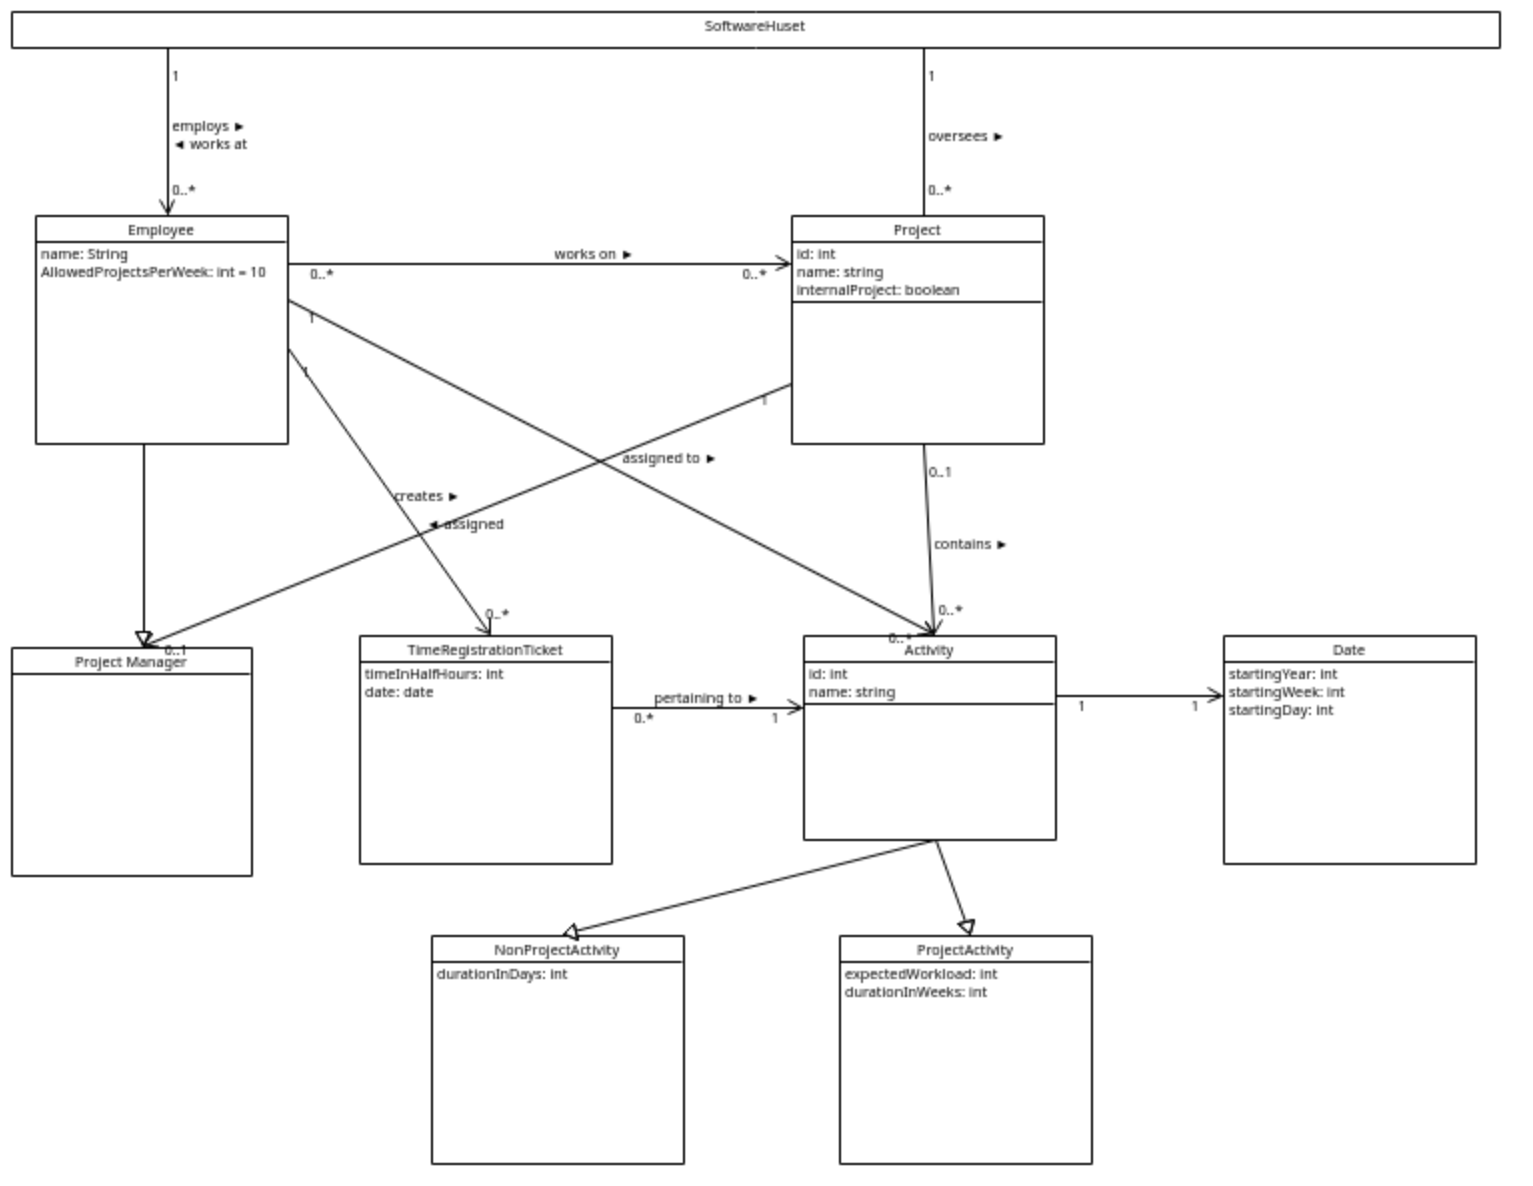
\includegraphics[width=\linewidth]{figures/ClassDiagram1.png}
    \caption{Class diagram}
    \label{fig:ClassDiagram}
\end{figure}


%Sekvensdiagrammer: Dette afsnit indeholder sekvensdiagrammer for de use casesfra afsnit 1d, s˚aledes at læseren f˚a et overblik over hvordan programmet bør udføredisse scenarier som tilhører til disse use cases. Der skal være sekvensdiagrammertil to use cases til hver gruppemedlem (et sekvensdiagram til hver hoved- ogalternative scenarier af hver use case).
\subsection{Sequence Diagrams}
This section contains sequence diagrams for all 10 Cucumber features found in section \ref{cucumber}.

\subsubsection*{Feature 1: Login to the system}
%1. Login to the system.


\subsubsection*{Feature 2: Create a new project}%Max 1
%2. Create a new project with a name and an ID.


\subsubsection*{Feature 3: Create non-project activity}
%3. Create a non-project activity and give it a starting date and expected duration.


\subsubsection*{Feature 4: Register time spent on activity}
%4. Register time spent working on an activity on a given day, even if I havent been specifically assigned to that activity.


\subsubsection*{Feature 5: Set project manager for a project}%Max 2
%5. Set myself as project manager - for a project that doesn't have a manager - and set starting week, duration and expected workload.


\subsubsection*{Feature 6: Edit project}
%6. Edit the project.


\subsubsection*{Feature 7: Create project activity}
%7. Create an activity in said project with starting date, duration and expected workload.


\subsubsection*{Feature 8: Assign an employee to a project activity}
%8. Assign an employee to an activity in said project.


\subsubsection*{Feature 9: Check available employees}
%9. View the employees who are available to be assigned during the time designated for an activity.


\subsubsection*{Feature 10: Create project report}
%10. Create a detailed report of my project, which showcases relevant metrics for evaluation.




%Afsnittet afsluttes med en kort diskussion hvor der, for eksempel, gøres rede for de valg derer truffet. Afsnittet kan ogs˚a omtale valg af algoritmer og datastrukturer.Slidserne i uge 6 anbefaler en process som kan bruges til at lave programdesign.
\subsection{Discussion}


 

\label{EndOfText}



\newpage
\section{References}
%\addcontentsline{toc}{section}{References}
\bibliography{document.bib} 
\bibliographystyle{IEEEtranN}

\newpage
\section{Appendix} \label{ch6}

\label{endOfDoc}
\end{document}



